\documentclass[10pt,a4paper]{report} 

\usepackage[utf8]{inputenc}
\usepackage{amsmath}
\usepackage{amsfonts}
\usepackage{amssymb}
\usepackage{graphicx}
\usepackage[final]{pdfpages}
\usepackage{stmaryrd}
\usepackage{listings}
\usepackage[hidelinks]{hyperref}
\usepackage[english]{babel}
\usepackage{color}
\usepackage{fancyhdr}
\usepackage{xcolor}
\usepackage{url}
\usepackage{sectsty}
\usepackage{etoolbox}
\usepackage{tikz}
\usepackage[acronym]{glossaries}
\usepackage{float}
\usepackage[bottom]{footmisc}
\usepackage[parfill]{parskip}
\usepackage{mathrsfs}
\usepackage{algpseudocode}
\usepackage{algorithm}
\usepackage{bbm}
\usepackage{subfig}
\usepackage{afterpage}
\usepackage[toc,page]{appendix}
\usepackage{multirow}
\usepackage[htt]{hyphenat}
\usepackage{todonotes}

% Abstract
\patchcmd{\abstract}{\null\vfil}{}{}{}

% Graphics and images
\graphicspath{{./images/}}

% Set headers to sans serif
\allsectionsfont{\sffamily}

% Defining colors for syntax highlighting
\definecolor{commentsColor}{rgb}{0.497495, 0.497587, 0.497464}
\definecolor{keywordsColor}{rgb}{0.000000, 0.000000, 0.635294}
\definecolor{stringColor}{rgb}{0.558215, 0.000000, 0.135316}

\lstset{aboveskip=20pt,belowskip=20pt}

% Source: https://denbeke.be/blog/programming/syntax-highlighting-in-latex/
\lstset{
  backgroundcolor=\color{white},
  basicstyle=\ttfamily\small,
  breakatwhitespace=false,
  breaklines=true,
  captionpos=b,
  commentstyle=\color{commentsColor}\textit,
  deletekeywords={...},
  escapeinside={\%*}{*)},
  extendedchars=true,
  frame=tb,
  keepspaces=true,
  keywordstyle=\color{keywordsColor}\bfseries,
  %language=Python,
  otherkeywords={*,...},
  numbers=left,
  numbersep=5pt,
  numberstyle=\tiny\color{commentsColor}, 
  rulecolor=\color{black}, 
  showspaces=false,
  showstringspaces=false,
  showtabs=false, 
  stepnumber=1, 
  stringstyle=\color{stringColor},
  tabsize=2, 
  title=\lstname,
  columns=fixed 
}

% Bibliography
%\bibliographystyle{unsrturl}
\bibliographystyle{alpha}


% Pagestyle
\pagestyle{fancy}

% Hyperlinks
\hypersetup{
  colorlinks=true,
  allcolors=black
}

% Headers
\fancyhf{}
\lhead[\textit{\leftmark}]{}
\rhead[]{\textit{\leftmark}}

\cfoot{\thepage}


\begin{document}

\title{
\vspace{-80px}

\includegraphics[width=5cm]{bfh-logo}\\
\vspace{80px}
\huge\textsf{\textbf{Implementation of a Real-time Streaming-based Terrain Level of Detail System}}\\
\vspace{40px}
\large{Bachelor Thesis
by\\}
\vspace{10px}
\Large{Amar Tabakovic\\}
\vspace{20px}
\large{
\textbf{Bern University of Applied Sciences}\\
  Engineering and Information Technology\\
  Computer Perception \& Virtual Reality Lab
\\
\vspace{15px}
\textbf{Supervisor}\\
Prof.~Marcus Hudritsch\\
\vspace{15px}
\textbf{External expert}\\
Dr.~Eric Dubuis}\\
\vspace{20px}
\today
}

\date{}
\maketitle

\begin{abstract}
Terrains are an important part of various practical applications of computer graphics, such as
video games, flight simulators and geographical information systems (GIS).
Since terrains are expensive to render, various terrain level of detail (LOD) approaches have been developed
over the last three decades.
Terrain LOD algorithms improve the performance of terrain rendering 
by applying various optimizations, such as rendering distant areas in a lower resolution,
not rendering areas out of view (view-frustum culling), and more.
Besides the rendering performance, another important aspect to terrain rendering is the size of terrain data.
Terrain data too large to fit entirely in memory must be streamed 
from the disk or over the network.

This thesis describes the implementation of a real-time streaming-based terrain LOD system,
which is capable of streaming in data from various providers based on the XYZ map tiling scheme.
The implemented terrain LOD algorithm is based on Chunked LOD by Ulrich TODO cite.



\end{abstract}

\tableofcontents

\listoftables
\listoffigures
\lstlistoflistings

\chapter{Introduction}
Terrains are an important part of many practical applications of 3D computer graphics.
They can be found in video games, simulation software and geographical information systems (GIS). 
Terrains are, however, due to their constant visibility and sheer size expensive to render.
Over the last three decades, efficient terrain rendering has been the topic of research
and numerous terrain rendering algorithms and approaches spawned. 

Another important problematic aspect of terrain rendering is the efficient 
and real-time storage, organisation and usage of terrain data. 
In order to support terrains which cannot fit entirely in 
memory, various terrain paging and streaming approaches 
were developed and published over the last few years as well.


\section{Goals of this Thesis}
% The goals of this thesis are split up into the \textit{must goals},
% \textit{should goals} and \textit{optional goals}.

% \subsection{Must Goals}
% Must goals are goals which the system to implement must 
% have, as otherwise this thesis cannot be considered sucecssful. TODO

% \paragraph{}

% \subsection{Should Goals}
% TODO

% \paragraph{}

% \subsection{Optional Goals}
% Optional goals are features which TODO

% The following goals can be considered optional goals.

% \paragraph{}

\section{Intended Readership}
The reader is assumed to be familiar with the basics of computer science,
C++ programming and 3D computer graphics.

\section{Structure of this Thesis}
This thesis is structured as follows:
\begin{itemize}
  \item Chapter 2 introduces the reader to various topics covered in this thesis, such as terrain LOD rendering. In addition, 
        basic terminology and notation is defined.
  \item Chapter 3 gives an overview of previous work conducted in the area of real-time terrain streaming and 
        a short recap of the preceeding project ``3D Terrain with Level of Detail''.
  \item Chapter 4
  \item Chapter 5
  \item Chapter 6
  \item Chapter 7
  \item Chapter 8
  \item Chapter 9
  \item Appendix A contains various artifacts related to the project management of this thesis.
  \item Appendix B contains the usage guide for Streaming-ATLOD with installation and building steps.
\end{itemize}

TODO dynamic links


\chapter{Theoretical Background}
This chapter describes some background information 
on computer graphics, terrain LOD and network programming.

\section{Notation and Terminology}
\subsection{Mathematical Notation}

\subsection{Terminology}

\section{Terrain Rendering}
Terrain rendering refers to the process of displaying the terrain on the screen.

\subsection{Data Representation}
Terrain data can be represented in a number of ways.

\subsection{Level of Detail}
\textit{Level of Detail (LOD)} is the concept of reducing the complexity of a mesh 
using various metrics to optimize rendering performance.
Such metrics include the distance of the mesh to the camera,
the dimensions of the mesh in screen-space and more.

Terrain LOD algorithms can be categorized as follows.

\paragraph{}

Some of the most important terrain LOD algorithms are summarized in 
chapter TODO.

\section{Terrain Streaming}
For visualizing very large terrains, 
the main memory is often not large enough to hold the entire terrain data.
In this case, terrain rendering systems often deploy 
\textit{terrain streaming} (also called \textit{terrain paging}), which refers to the concept of dynamically 
loading and offloading terrain data from the disk or from a network, such as the internet.


\chapter{Previous Work}
This chapter aims to outline some already existing approaches and 
work. 
First, an overview of algorithms, literature and software systems for streaming-based terrain rendering is given,
in which some of their central ideas are outlined.
Afterwards, the author's 
predecessor project on basic terrain LOD rendering is summarized.

\section{Terrain LOD Algorithms}
In this section, a few terrain LOD algorithms are introduced. 
The reasoning behind choosing these algorithms is that 
StreamingATLOD relies on a few techniques introduced by these 
algorithms.
Older terrain LOD algorithms which rely on continuous LOD,
such as ROAM \cite{roam} or SOAR \cite{soar} are left out,
since they are not relevant for this thesis.

\subsection{Geometrical MipMapping}
\textit{Geometrical MipMapping} (also called \textit{GeoMipMapping}) is a discrete terrain LOD algorithm 
introduced by de Boer \cite{geomipmapping} in 2000. The idea is 
to split up the terrain into square blocks of side length
$2^n + 1$ for some $n \in \mathbb{N}$ and to create 
multiple meshes for different LOD resolutions of the same block. Each block 
has an AABB for view-frustum culling and a 
maximum geometrical error for the LOD level computation.

A quadtree is used for accelerating view-frustum culling 
in which the blocks are stored at the leaf nodes.
Cracks between adjacent blocks with different LOD levels 
are prevented by ommitting the crack-causing vertices 
from the higher resolution mesh.

GeoMipMapping can be implemented with streaming by traversing 
all terrain blocks on the disk and generating a quadtree that stores 
the AABB of all blocks in the leaf nodes. The blocks required for rendering 
are then loaded using the AABBs stored in said quadtree.

The main advantage of GeoMipMapping is that it is simple to understand 
and implement. The main disadvantage is that it scales poorly, 
since each block has the same size, making extremely large 
terrains more difficult to implement without special modifications.

\subsection{Chunked LOD}
\textit{Chunked LOD} is a hierarchical terrain LOD algorithm 
introduced by Ulrich in the year 2002 \cite{chunkedlod}. 
The idea of Chunked LOD is to organize the terrain 
into a quadtree of chunks.
Each chunk represents a section of the terrain at a particular LOD level,
where the LOD level is given by the chunk's depth in the quadtree.
Each non-leaf chunk has four children, where each child chunk
represents a fourth of its parent's area, but in twice the resolution.
The root chunk represents the entire terrain at the lowest resolution.

The heightmap and textures are preprocessed and organized 
into their respective chunks.
During preprocessing, the section of the heightmap inside 
a chunk's bounds is compressed into a TIN.

Cracks between adjacent chunks with different LOD levels are 
hidden by rendering skirts around each chunk. Popping artifacts are prevented 
through geomorphing.
Chunked LOD supports streaming
and is designed to render the already available data in case 
the requested data is not loaded yet.

The main advantage of Chunked LOD is that 
it scales well and allows for massive terrains to be rendered
thanks to its hierarchical nature. The main disadvantage 
is that it requires some lengthy preprocessing of the terrain data.

\subsection{Geometry Clipmaps}
\textit{Geometry Clipmaps} is a discrete terrain LOD algorithm 
introduced by Hoppe and Losasso in 2003. A follow-up GPU-based 
variant of Geometry Clipmaps (called \textit{GPU-based Geometry Clipmaps}) was published by Hoppe and Asirvatham \cite{gpugeomclipmaps}
in the year 2004. In this subsection, GPU-based Geometry Clipmaps will be 
introduced.

The idea of GPU-based Geometry Clipmaps is to render a ring of constant grid-like flat meshes
centered around the camera and to displace the height values of the meshes in the vertex shader
using a heightmap that was loaded in advance as a texture on the GPU, a concept which has 
since been dubbed \textit{heightmap displacement}.
The scale of the meshes increases the further away from the camera they are,
resulting in fewer vertices for distant areas.

Cracks are avoided by rendering degenerate triangles
and popping artifacts are avoided through geomorphing in the vertex shader.
At close distances, the terrain is augmented with procedural detail 
generated in the vertex shader.

Hoppe and Asirvatham did not discuss streaming of terrain data.
Instead, they mainly relied on texture compression,
with which they compressed a 20-billion sample heightmap of the United States
into 355 MB and decompressed required sections at runtime for rendering.

The main advantage of GPU-based Geometry Clipmaps is that very little 
memory is used for the meshes thanks to heightmap displacement. The meshes only need to be defined 
once at start up and stay constant throughout the runtime.
The main disadvantage is that GPU-based Geometry Clipmaps 
does not incorporate height for LOD,
since the meshes are always centered around the camera.

\section{Reference Books}
\subsection{3D Engine Design for Virtual Globes}
The book \textit{3D Engine Design for Virtual Globes} by Cozzi and Ring \cite{3denginedesignforvirtualglobes}
is a reference book for various topics related to globe rendering. It includes 
chapters on mathematical basics of geographic coordinate systems,
terrain rendering basics, handling multithreaded rendering, 
solving precision issues and more.

\subsection{Level of Detail for 3D Graphics}
Subchapter ``7.2.5 Paging, Streaming, and Out of Core''
in the the book \textit{Level of Detail for 3D Graphics} \cite{lodfor3dgraphics} 
by Luebke et al.~describes some basic background, existing approaches and relevant publications 
related to terrain rendering and streaming. 

\section{Video Games and Game Engines}
\subsection{Microsoft Flight Simulator}
\textit{Microsoft Flight Simulator} is a video game developed by Asobo Studio and released in 2020.
The video game allows the player to fly on the entire earth and uses various 
data sources for representing the earth as accurately as possible.
It received high praise for its realism and immersion.

At the GDC 2022, Fuentes presented the terrain system of Microsoft Flight Simulator,
in which he described the data organization, system architecture, rendering process and many more aspects \cite{msflight}.
The terrain system utilizes a hierarchical LOD approach based on quadtrees and renders 
skirts to hide cracks, similarly to Chunked LOD.
It uses a large number of sources for height data, TINs, overlay texturing, vegetation, bodies of water, cities
and more. The data and its states are managed with a complex state-machine-based marker system,
where each piece of data of a tile (such as height data, TIN, etc.) is a state machine.
It also utilizes Microsoft Azure cloud for computing road data, tree masks and other features.

\section{Globe Renderers}
\subsection{Google Earth}
\textit{Google Earth} is a 3D globe viewer developed by Google 
released in the year 2001 and is most likely the 
most well-known example of a globe renderer.
It is capable of rendering the Earth by utilizing a number of data sources 
for its imagery and height data. 
Google Earth supports adjustable cache sizes for the disk cache and the memory cache.

\subsection{OpenWebGlobe}
\textit{OpenWebGlobe} \cite{openwebglobe} is a software development kit (SDK)
developed by the Institute for Geomatics at the 
University of Applied Sciences of Northwestern Switzerland. 
It is written in JavaScript and 
WebGL and designed for rendering 3D globes on web browsers. 
The source code of OpenWebGlobe is open source.

OpenWebGlobe's terrain data is preprocessed into TINs using 
a large-scale Delaunay triangulation using raw height data and subsequently organized into 
XYZ tiles. The triangulation was performed on a 
large-scale cluster of computers.

The Earth is rendered using a Chunked LOD-based 
hierarchical LOD algorithm using the preprocessed TINs 
and overlay textures served from web servers.
Multiple height and overlay layers are supported.

\subsection{Cesium}
\textit{Cesium Geospatial} is a company developing 
globe-rendering-related software.
Their open-source JavaScript and WebGL SDK 
\textit{Cesium JS} also uses a hierarchical 
LOD algorithm. For terrain data representation, they developed the
\textit{quantized-mesh} file format 
specifically designed for streaming.

\section{Review of Project 2 -- 3D Terrain with Level of Detail}
This thesis is the logical continuation of 
the author's preceeding project ``3D Terrain with Level of Detail'' \cite{p2}
as part of the project course ``Project 2'' at the Bern University of Applied Sciences.
In said project, the basics of terrain rendering and existing approaches for terrain LOD were 
studied and a simple terrain renderer named \textit{ATLOD} was developed.
Terrain rendering with streaming was explicitly left out of scope of the preceeding project.

\subsection{Summary of the Implemented Terrain LOD Algorithm}
The implemented LOD algorithm is mainly based on GeoMipMapping \cite{geomipmapping},
but performs the rendering with heightmap-displacement in the vertex shader,
as introduced by GPU-based Geometry Clipmaps \cite{gpugeomclipmaps}.
The terrain gets split up into blocks of size $blockSize = 2^n + 1$ for some $n \in \mathbb{N}$.
Each block contains information related to a particular section of terrain, such as current LOD level, its world-space center point, 
its AABB, current border permutation.
A single grid-like flat mesh of side length $blockSize$ is stored on a single global vertex and index buffer.
This flat mesh will be used to render every block at runtime.
The indices are stored such that the flat mesh is split into its center and border area. 
The border area is defined in a special manner in order to prevent cracks from occuring.

The first part of the index buffer 
contains indices of the center area at every LOD resolution, from highest to lowest, 
and the second part of the index buffer contains the indices of the border area 
at every LOD resolution and for every of the $2^4=16$ possible border permutations. 
A border permutation is a 4-tuple $(l,r,t,b)$ (the variables corresponding to left, right, top and bottom) 
representing a border area, set up such that each element of the 4-tuple is set to 1 if the neighboring block 
on the corresponding side has a lower LOD level, otherwise 0. The maximum difference 
in LOD level between any two neighboring blocks must be 1.
The heightmap is stored as a texture object on the GPU.

At runtime, in a first step the LOD level and current border permutation of each block 
is updated. The new LOD level is calculated using the distance between the camera 
and the block's center point.
In a second step, each block is intersected with the view-frustum 
and if the block's AABB is inside the view-frustum, the block gets rendered with two draw-calls,
one for the center area and one for the border area.

In the vertex shader, each vertex of the flat mesh gets translated by the block's world-space center point
and the heightmap is sampled for a height value with the $(x,z)$ coordinates of the vertex, 
which is then used to displace the $y$-coordinate.
In the fragment shader, the overlay texture is applied and Phong shading is calculated.
The normal vectors for Phong shading are calculated using the four orthogonally neighboring points 
in the heightmap. Finally, a simple distance fog is applied.

\subsection{Results}
The renderer worked well on the tested hardware (Apple Intel MacBook Air 2020), 
consistently rendering around 60 frames per second with a 
$14000 \times 14000$ terrain. A screenshot of a rendered terrain 
is shown in figure \ref{fig:atlod}.

\begin{figure}[H]
  \centering
  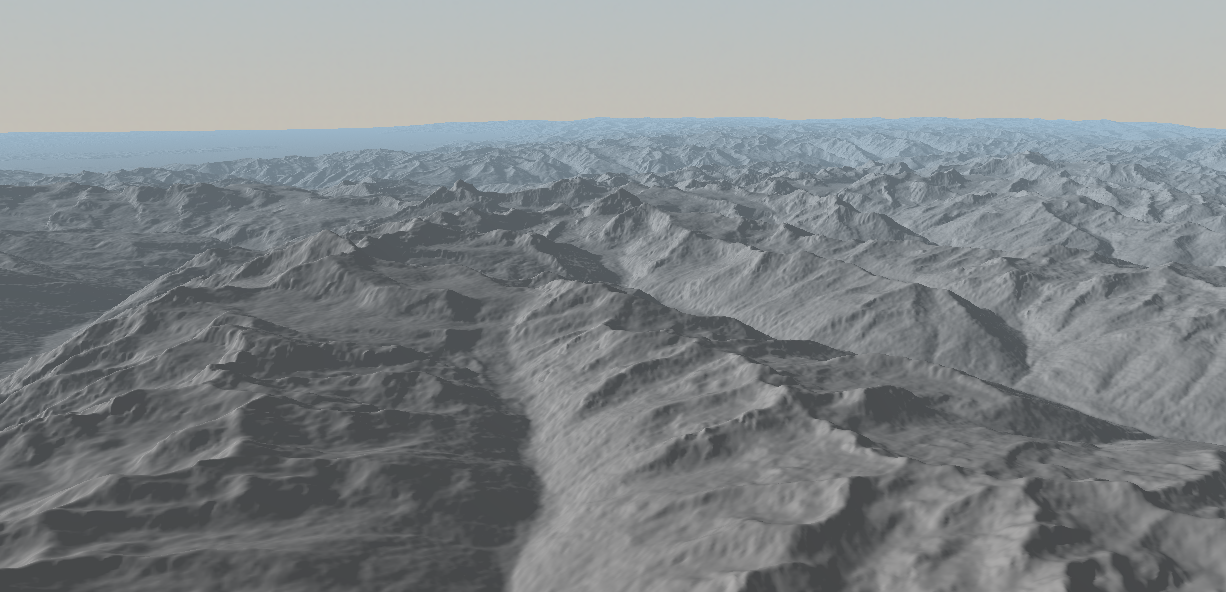
\includegraphics[width=1\textwidth]{atlod.png}
  \caption{Screenshot of a terrain rendered in ATLOD.}\label{fig:atlod}
\end{figure}

The main strengths of the implemented terrain LOD algorithm are
its low GPU memory usage, since each block uses the same mesh,
and its simplicity to understand.

Some improvement points in terms of visual and rendering performance 
were to render the terrain with geomorphing to avoid popping artifacts, \textit{instanced rendering} for
reducing the number of draw calls and improving 
view-frustum culling by organizing AABBs in a quadtree.

The most important missing technical feature, however, was support for 
streaming, which would allow for even larger terrains 
to be rendered. 
\chapter{StreamingATLOD}
This chapter describes the implementation of \textit{StreamingATLOD} (\textbf{Streaming-A}ssisted 
\textbf{T}errain \textbf{L}evel \textbf{o}f \textbf{D}etail (Renderer)).

\section{Used Technologies}
StreamingATLOD is written in C++17 and OpenGL 3.3. For compiling build files,
CMake (minimum version 3.5) is used. ATLOD uses the following third-party
libraries:
\begin{itemize}
  \item GLM:
  \item GLEW:
  \item GLFW:
  \item Dear ImGui:
  \item STB:
  \item libwebp:
\end{itemize}


\section{Terrain LOD Algorithm}
The implemented terrain LOD algorithm is based on \textit{Chunked LOD} by Ulrich TODO cite.
Chunked LOD organizes the terrain into a quadtree, where each node represents a section of the terrain with data,
such as heightmap and textures. Chunked LOD and its derived approaches are used in other large-scale terrain rendering systems, such as 
TODO cite.

\subsection{Quadtree Organisation}


\subsection{Terrain Mesh}

\subsection{Crack Prevention}

\section{Map Projection}

\section{Data Streaming}

\section{Tile Caching}

\chapter{Results}
\section{StreamingATLOD}

\section{Terrain Streaming Server}
\chapter{Discussion}
\chapter{Conclusion}

\bibliography{bibliography}
\addcontentsline{toc}{chapter}{Bibliography}

\appendix
\chapter{Time Schedule}
\begin{figure}[H]
  \centering
  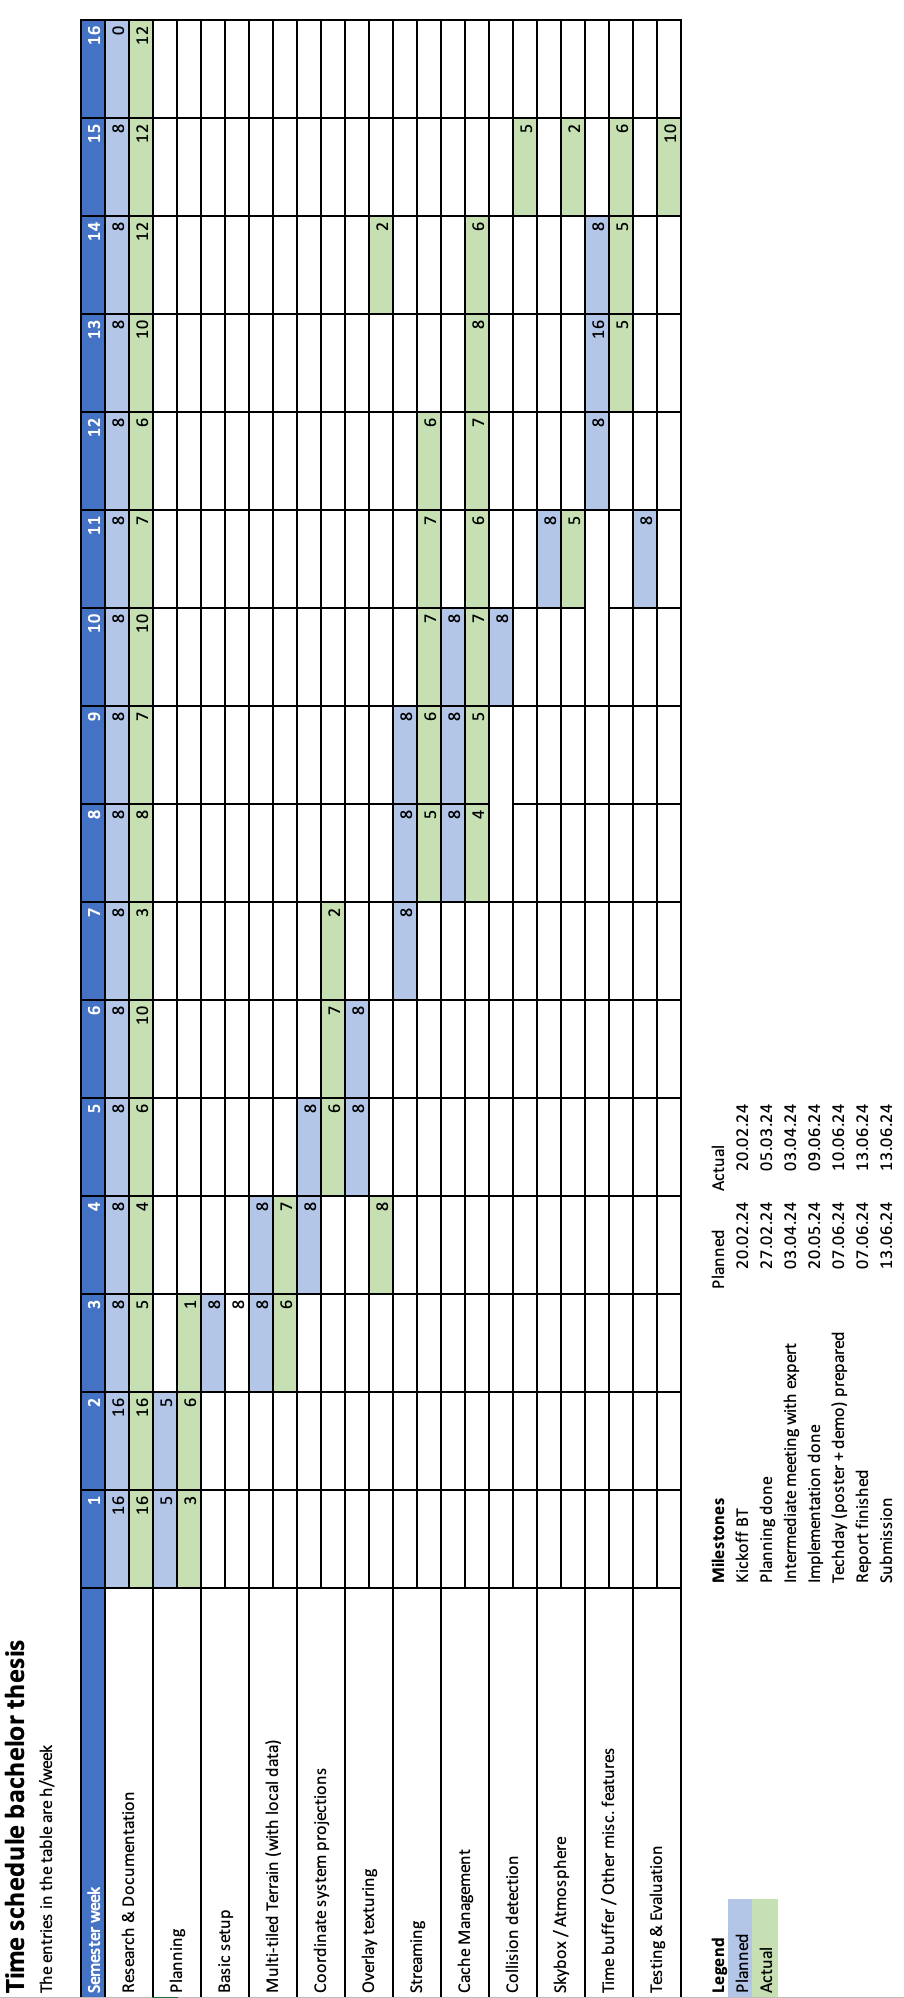
\includegraphics[width=0.6\textwidth]{time-plan.png}
  \caption{The time schedule of this thesis.}\label{fig:time-plan}
\end{figure}


\end{document}
